\documentclass[9pt]{IEEEtran}

\usepackage[english]{babel}
\usepackage{graphicx}
\usepackage{epstopdf}
\usepackage{fancyhdr}
\usepackage{amsmath}
\usepackage{amsthm}
\usepackage{amssymb}
\usepackage{url}
\usepackage{array}
\usepackage{textcomp}
\usepackage{listings}
\usepackage{hyperref}
\usepackage{xcolor}
\usepackage{colortbl}
\usepackage{float}
\usepackage{gensymb}
\usepackage{longtable}
\usepackage{supertabular}
\usepackage{multicol}

\usepackage[utf8x]{inputenc}

\usepackage[T1]{fontenc}
\usepackage{lmodern}{}
\input{glyphtounicode}
\pdfgentounicode=1

\graphicspath{{./figures/}}
\DeclareGraphicsExtensions{.pdf,.png,.jpg,.eps}

% correct bad hyphenation here
\hyphenation{op-tical net-works semi-conduc-tor trig-gs}

% ============================================================================================

\title{\vspace{0ex}
Optical flow}

\author{Marko Medved\vspace{-4.0ex}}

% ============================================================================================

\begin{document}

\maketitle

\section{Introduction}
In this assignment, the mean shift method was first implemented and then
 used to develop a tracker, which was tested on the VOT14 dataset. The model's
  performance was evaluated using different parameters. The tracker was 
  further improved by introducing additional weights for the histogram, 
  with the weights selected based on the tracked object's background.
\section{Experiments}
\subsection{Mean shift mode seeking on the given example}
The Mean Shift method was tested using several different parameters to assess 
its performance. Firstly, the kernel size, which determines the region over which
 the probabilities for making a step are calculated, was varied. Additionally, 
 different starting positions on the density function were considered to evaluate 
 how the initial location affects the results. Lastly, three convergence criteria
  were tested to determine when the iteration should stop: the first, based on step
  size, stops the iteration when the calculated movement is smaller than one pixel; 
  the second, using Euclidean distance, halts the process when the distance between 
  consecutive positions is less than 2 units; and the third, based on change in
   probability, terminates the iteration when the change in the probability 
   distribution is minimal, indicating convergence.

  In Figure~\ref{fig:mode_seeking}, we observe how different combinations of
   these parameters affect convergence. A larger kernel size leads to faster
    convergence, as the calculated steps are generally larger. However, when the 
    kernel size is too small, the algorithm fails to converge to the local maximum 
    because the calculated steps become smaller than a pixel. On the other hand, 
    using an excessively large kernel can also prevent convergence to the local
     maximum, as illustrated by the example with the largest kernel size.

     The starting position is also crucial, as it directly influences the algorithm's
      behavior. If the starting point is located where there is little to no
       probability in the surrounding area, the algorithm will fail to make any 
       steps. Additionally, for functions with multiple local maxima, the starting
        position determines which maximum the algorithm will converge to. 

        Lastly, among the different types of convergence criteria, the sub-pixel 
        step method is generally the most consistent, although it tends to be the
         slowest. It's also worth noting that the "small change in probability" 
         criterion may not always be the best choice, especially if the probabilities 
         change insignificantly at the start, as it can lead to premature convergence.

\subsection{Mean shift mode seeking on custom examples}

\begin{figure}[h]
    \centering
    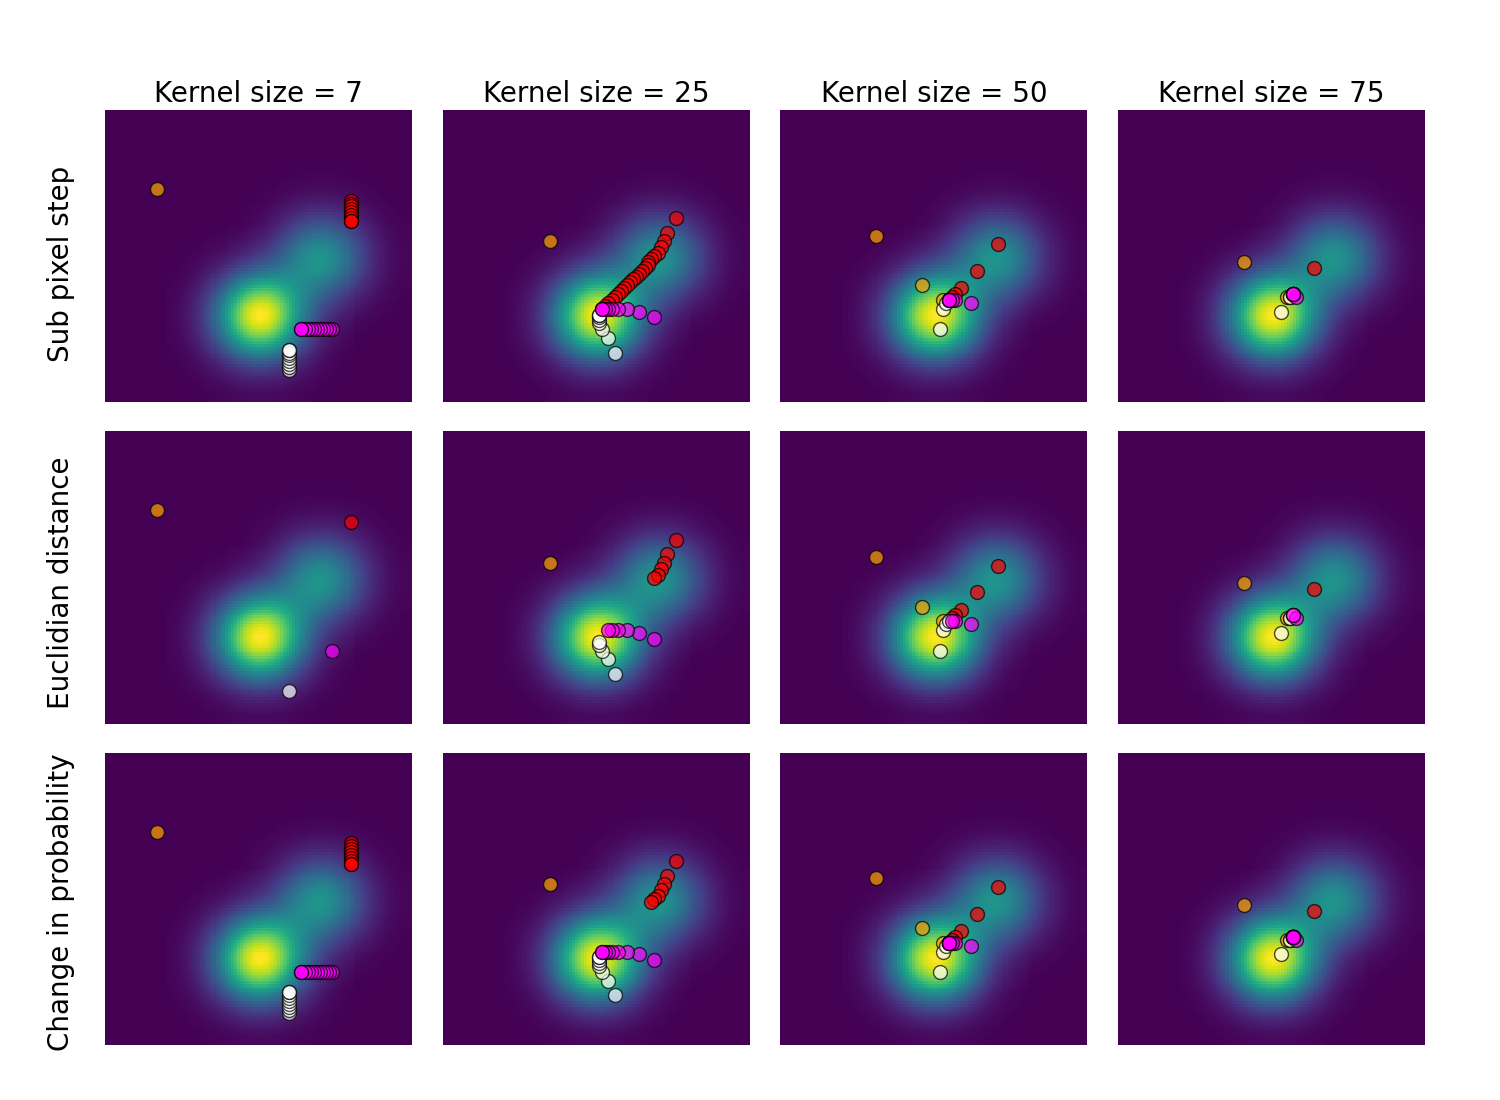
\includegraphics[width=0.99\columnwidth]{figures/mode_seeking.png}
    \caption{Comparison of the mean shift method with different kernel sizes, convergence
    criteria and starting positions}
    \label{fig:mode_seeking}
\end{figure}


\bibliographystyle{IEEEtran}
\bibliography{bibliography}

\end{document}
